%!TEX root = ../../../thesis.tex
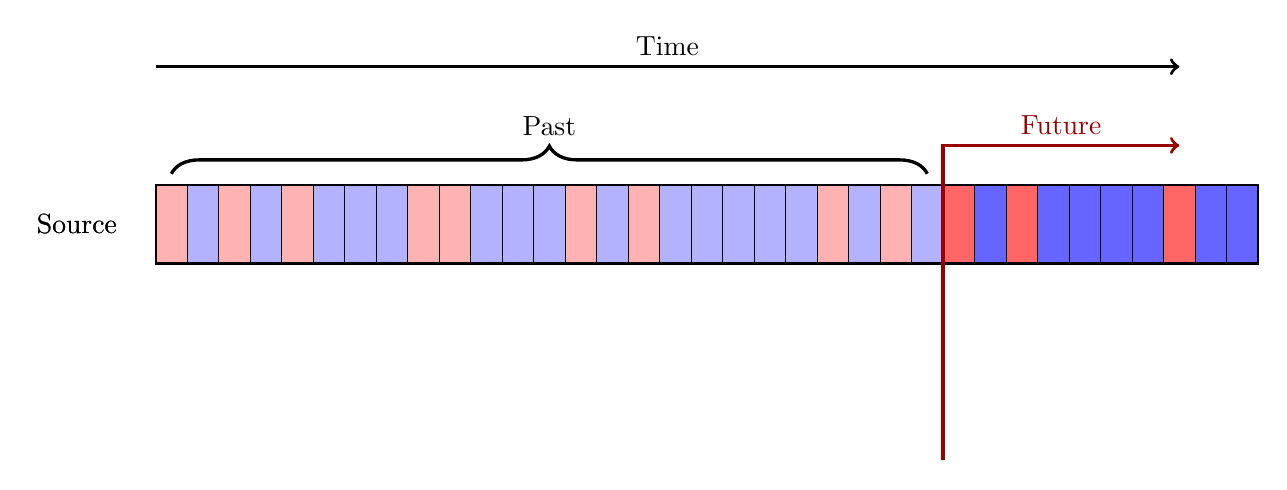
\begin{tikzpicture}
	
	%% TOP EVENTS
	
	\node at (-1, 0.5) {Source};
	
	% Events
	% Past Events
	\draw [thick, fill = blue!30!white] (0,0)  rectangle (10,1)  ;
	\foreach \x in {0, 0.8, 1.6, 3.2, 3.6, 5.2, 6, 8.4, 9.2}
	{
		\fill[red!30!white] (\x ,0) rectangle ++(0.4,1);
	}
	
	% Future Events
	\draw [thick, fill = blue!60!white] (10,0) rectangle (14,1) ;
	\foreach \x in {10, 10.8, 12.8}
	{
		\fill[red!60!white] (\x,0) rectangle ++(0.4,1);
	}
	
	% Redraw Main Rectangle
	\foreach \x in {0,...,34}
	{
		\draw [very thin] (0.4*\x,0)  rectangle ++(0.4,1);
	}
	\draw [thick] (0,0) rectangle (14,1) ;
	
	
	
	%%ORANGE EVENTS
	
	\node at (-1, 0.5) {Source};
	
	% Events
	% Past Events
	\draw [thick, fill = blue!30!white] (0,0)  rectangle (10,1)  ;
	\foreach \x in {0, 0.8, 1.6, 3.2, 3.6, 5.2, 6, 8.4, 9.2}
	{
		\fill[red!30!white] (\x ,0) rectangle ++(0.4,1);
	}
	
	% Future Events
	\draw [thick, fill = blue!60!white] (10,0) rectangle (14,1) ;
	\foreach \x in {10, 10.8, 12.8}
	{
		\fill[red!60!white] (\x,0) rectangle ++(0.4,1);
	}
	
	% Redraw Main Rectangle
	\foreach \x in {0,...,34}
	{
		\draw [very thin] (0.4*\x,0)  rectangle ++(0.4,1);
	}
	\draw [thick] (0,0) rectangle (14,1) ;
	
	
	
	% Future
	\draw [red!60!black, very thick, shorten >= -0.6pt]        (10,-2.5 ) -- (10,1.5);
	\draw [red!60!black, very thick, ->] (10,   1.5)  -- (13, 1.5)   node[midway, above] {Future} ;
	
	% Time Arrow
	\draw [very thick, ->] (0,2.5) -- (13,2.5) node[midway, above] {Time} ;
	
	% Past brace
	\usetikzlibrary{decorations.pathreplacing}
	\draw [very thick, -, draw=black, decorate, decoration={brace,amplitude=10pt,mirror,raise=4pt} ] (9.8,1) -- (0.2,1)
	node[midway, above, yshift = 14pt] {Past} ;
	
	\end{tikzpicture}